\section{Preliminary Remarks}\label{body_prelim}


%# EXAMPLE OF FORMULA
%# \begin{quotation}
%# \centering
%#    \( A_t = \delta_t + (\gamma \lambda)\delta_{t+1} + ... + (\gamma \lambda)^{T-t+1} \delta_{T-1} \)
%# \end{quotation}


%# EXAMPLE OF PSEUDOCODE
%# \begin{algorithm}
%# \caption{Pseudocode Implementierung des PPO, Actor Critic }
%# \begin{algorithmic}
%#
%# \WHILE{$i < iterations $}
%# 	\WHILE{$actor < N$}
%# 		\STATE  run policy $ \pi_{\theta_{old}} $ in environment for T steps
%# 		\STATE compute advantage estimates $ A_1, ..., A_T$
%# 	\ENDWHILE
%# 	\STATE optimize surrogate objectiv $ L(\theta) $ with K epochs and minibatches of size $ M \leq NT $
%# 	\STATE $ \theta_{old} \leftarrow \theta $
%# \ENDWHILE
%#
%# \end{algorithmic}
%# \end{algorithm}


%# EXAMPLE OF Figure
%# \begin{figure}[bp!]
%#
%#    \captionsetup{width=0.45\linewidth}
%#     \centering
%#     \begin{minipage}{0.45\linewidth}
%#         \centering
%#         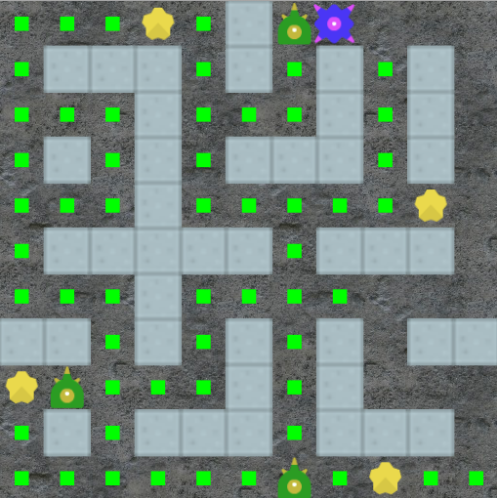
\includegraphics[scale=0.3]{abb/ss_chaser_gros}
%#         \caption{Chaser - unskaliert.}
%#         \label{fig:pic_chaserGros}
%#     \end{minipage}
%#     %\hfill
%#     \begin{minipage}{0.45\linewidth}
%#         \centering
%#         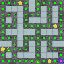
\includegraphics[scale=2.35]{abb/ss_chaser_klein}
%#         \caption{Chaser - herunterskaliert.}
%#         \label{fig:pic_chaserKlein}
%#     \end{minipage}
%#     %\caption{Chaser Environment - links unskaliert, rechts skaliert}
%# \end{figure}

%# EXAMPLE OF LIST OF ITEMS
%#   \begin{itemize}
%#     	\item \emph{idle-State}: Dieser State ist ein Übergangsstate, in welchem die Geister auf dem Spielfeld erscheinen. Nach $t_1$ Sekunden wird der Geist automatisch in den tödlich-State überführt. Dieser State ist optisch durch ein eigenes Sprite differenziert. Geister in diesem State bewegen sich nicht und können dem Jäger noch nicht schade.
%#   	\item \emph{tödlich-State}: Eine Berührung des Jägers mit einem Geist in diesem State beendet die Episode. Die Geister laufen in diesem State zufällig und ziellos.
%#   	\item \emph{verletzlich-State}: Geister können vom Jäger in diesem State gefressen werden. Sammelt der Jäger einen großen Orb ein, überführt er die Geister damit in diesen State. Dieser State ist optisch durch ein eigenes Sprite differenziert. Dieser State führt nach $t_2$ Sekunden wieder in den tödlich-State, wenn der Geist nicht gefressen wird.
%#   	\item \emph{killing-State}: Ist ein Geist zwei oder weniger Felder vom Jäger entfernt, so wird der Geist in diesen State überführt. In diesem State läuft der Geist nicht mehr in zufällige Ricthungen, sondern zielstrebig auf den Jäger zu.
%#   \end{itemize}

%# EXAMPLE OF TABLE
%# \begin{table}[bp!]
%# \centering
%# \begin{tabular}{|c|c|c|}
%# \hline
%# \textbf{Parameter} & \textbf{Wert} & \textbf{Beschreibung} \\
%# \hline
%# \textbf{a} & 1 & Beschreibung \\
%# \hline
%# \textbf{b} & 2 & Beschreibung \\
%# \hline
%# \textbf{c} & 3 & Beschreibung \\
%# \hline
%# \end{tabular}
%# \caption{Tabellenbeschriftung}
%# \end{table}




%\cite{espeholt2018impala}
%Dieses Paper enthält eine brauchbare Grafik zum erläutern der Impala architektur
%\cite{espeholt2019seed}











\newpage
